\section{Task Prompts, Inputs, and Execution Conditions}\label{app:B}
\subsection{Three independent static routes}
R independently answers a fixed relation list from the assigned drawings and target descriptions. A independently constructs an executable world from the same core evidence. Its answers are then read from the submitted world. B constructs a world with the additional correct determinate relation list. R is not used to initialize A, and A is not used to initialize B. The pairing unit is the same building, product configuration, and query, not an assumed shared hidden reasoning state.

This design distinguishes two questions. R versus A asks whether a configuration performs similarly when answering and constructing. A versus B asks whether correct relation input improves the construction. A lower A score does not prove that one particular generation internally knew a correct answer and lost it during serialization. A B failure shows that supplied relations were not successfully realized under the output contract; its cause can still be parsing, representation, geometry, identity, or localization.

\begin{table}[htbp]\centering\small
\begin{tabular}{p{.13\linewidth}p{.35\linewidth}p{.40\linewidth}}\toprule
Route & Allowed scientific evidence & Required output\\\midrule
R & Assigned pages, locators, fixed queries & Relation-answer JSON with source references\\
A & Same core evidence; world Schema and contract & One executable world; no direct answer table\\
B & A inputs plus correct determinate relation values & One executable world realizing the supplied relations\\\bottomrule
\end{tabular}
\caption{The primary routes. Neither model outputs nor organizer coordinates are passed across routes. Qwen R's additional generic Schema is an interface difference described in Appendix~\ref{app:F}.}\label{tab:B-routes}
\end{table}

\subsection{Exact prompts and a complete bounded example}
The release includes the saved prompt text for each route and condition. Paths are translated to package-relative paths in the portable copy. The scientific wording, query values, and image pixels are retained. Listings~\ref{lst:B-common}--\ref{lst:B-task} give the common N2 instruction and the complete compact Rock Schoolhouse task specification. The listings use portable formatting for readability; the saved text files are the exact wording record. A/B additionally receive the frozen Schema. The B relation supplement is separate from the task file and is included with the example.

\lstinputlisting[caption={N2 common scientific and execution instruction, shared by the example routes.},label={lst:B-common}]{examples/N2_COMMON.txt}

\subsection{Route-specific final instructions}
The common prompt ends with an assigned task identifier and one of the following instructions. These are transcribed from the saved N2 prompts. R's answer wrapper is fixed; geometry is not requested in R.
\begin{lstlisting}
R: Independently answer the fixed questions from these images.
Return one plain JSON object:
{"schema":"topoworld_relation_answers_v1","case_id":"C02_ut0027",
 "answers":[{"query_id":"...","value":"TRUE|FALSE|UNKNOWN|NOT_FOUND or numeric value",
 "evidence":[{"view_id":"...","description":"..."}]}]}.
Include every query once. Do not build a world.

A/B: Construct one executable world matching the supplied
topoworld_executable_v1 Schema and case_id. Include task_bindings
for every target role and observations for every requested anchor.
Return plain JSON, not a direct answer table.

A: Infer the target structure from the images and neutral task
locators. No correct relation table or previous output is supplied.

B: The given_correct_relations are independently source-checked
input. Realize these relations in actual geometry/identity
assignments, without access to reference coordinates.
\end{lstlisting}

\lstinputlisting[caption={Complete scientific task content for the two-page C02 example. Paths are relative; image hashes are retained in the machine-readable task. No reference answer is in this file.},label={lst:B-task}]{examples/C02_TASK_COMPACT.json}

\begin{figure}[htbp]\centering
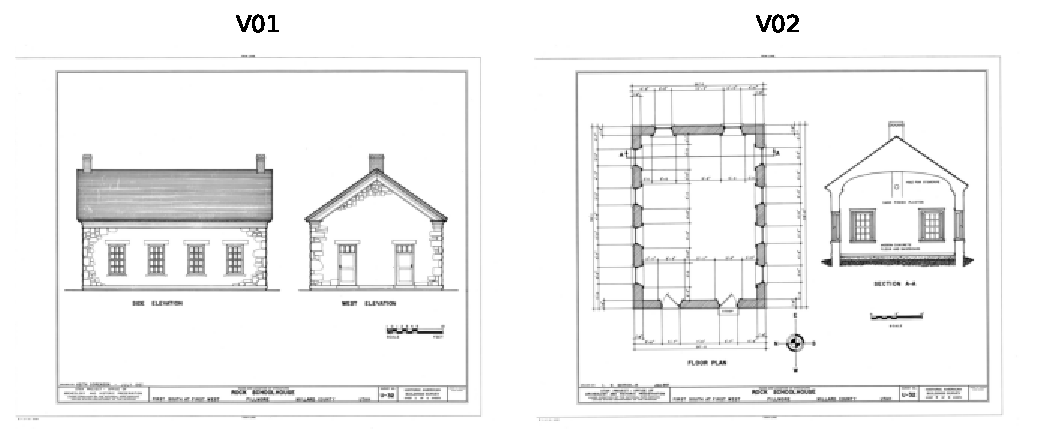
\includegraphics[width=.98\linewidth]{figures/C02_all_inputs.pdf}
\caption{All assigned image pages for the complete C02 example. The package includes these PNGs at their original task resolution. The printed overview is reduced for space and is not an alternative model input.}\label{fig:B-images}
\end{figure}

\paragraph{B-only relation supplement.} For this example, B additionally receives \texttt{Q01=TRUE}, \texttt{Q02=TRUE}, \texttt{Q03=TRUE}, \texttt{Q04=TRUE}, \texttt{Q05=TRUE}, \texttt{Q06=FALSE}. R and A do not receive this list. The full saved B task retains its machine-readable predicate arguments and values.

\subsection{Input conditions and output limits}
v1 supplies semantic target descriptions. N2 uses neutral IDs, point locators, and class hints; the input difference is intentional and must not be averaged away. CS1 uses neutral anchors with additional object-unit hints needed for complex multi-run and local-step questions. All three use the same bounded executable primitive family, but the content and difficulty of the tasks differ.

The construction contract limits the first output to 42,000 characters and 60 entities. It permits boxes, finite box unions, axis-aligned straight stair runs, and explicit unknown geometry. It asks for a shared coordinate frame, stable physical instances, observations with image boxes, target bindings, and evidence support. Unmeasured dimensions may be hypothetical completions. Such a completion must preserve supported relations, disclose uncertain parameters, and avoid claiming an exact recovered metric building.

The full Schema is supplied as a separate machine-readable file. It checks fields and types, not whether the building is correct. A syntactically valid response can fail the Schema; a Schema-valid response can still fail compilation or geometry. Conversely, an unknown geometry field can be valid while earning neither determinate readout nor required coverage.

\subsection{Codex context and tool boundary}
Each GPT task uses a fresh configuration-specific context derived from a READY-only seed, with the recorded product alias and \texttt{xhigh} setting. The seed carries the task rules, not a previous building answer. Each independent route receives its own job. The instructions allow assigned file/image reads, crops from the same pixels, and saving the first output. They prohibit other outputs, private references, external search, solver calls, evaluator feedback, and delegated solving.

This is an instruction-level boundary, not an operating-system filesystem sandbox. The audit retains observed departures. They include historical delegation-related missing outputs, one N2 computer-state request returning a locked/empty display, and CS1 access to an older public contract and a listing of temporary crop names. These events do not establish that hidden answers were read. They do prevent a claim that every run used an enforced identical sandbox. The primary results retain these allocations; sensitivity records identify their qualification.

Product names and effort settings are recorded as observed settings. The desktop interface does not provide a verified immutable neural checkpoint for each alias. We therefore report fixed Codex product configurations. We do not treat the eight configurations as eight independent provider families or equate their effort label with a measured floating-point budget.

\subsection{First-output policy and failed delivery}
The first complete response is saved before evaluation. The parser does not add a missing comma, deduplicate a key, fill a missing world, or infer an omitted endpoint. Empty, missing, malformed, oversized, and Schema-invalid outputs remain separate outcomes. A standard-path failure is not replaced using a better artifact discovered elsewhere. The independently retained wrong-location diagnostic remains outside the primary score.

All allocated determinate opportunities remain in the main denominator. A failed world can make several queries unevaluable; those are several missed obligations, not several independently established cognitive errors. A common-valid paired analysis is reported alongside the full denominator to isolate content differences after excluding delivery and format failures. It still includes geometric errors within valid outputs.

The task forbids an automatic generate--check--retry loop. The historical feedback pilot and evidence-revision stages have their own explicitly bounded designs. Their additional feedback is not retroactively allowed for the primary A/B routes. Repeating the deterministic scorer in the release changes no model response and is not a new attempt.
